%! TEX root = ../outline.tex
% ------------------------- TH definitions ----------------------- %
\section{Subcooled Boiling and DNB}

The relationship between the surface temperature of an internally heated object and the heat flux from the surface into the surrounding fluid is shown in figure \ref{fig:boiling_curve}.

\begin{figure}[H]
    \centering
    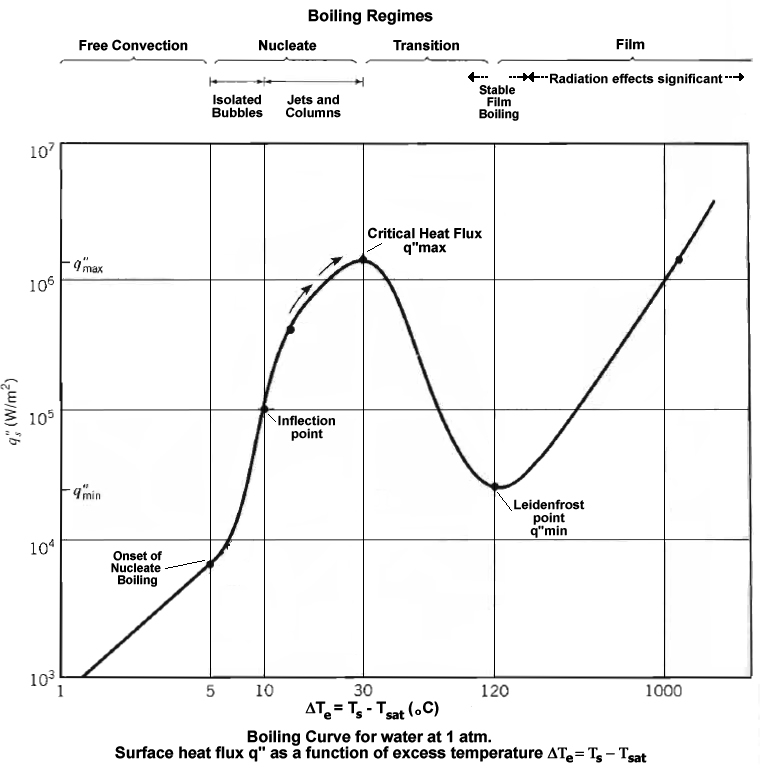
\includegraphics[width=0.7\linewidth]{../proposal/images/boiling_curve}
    \caption{Boiling curve.}
    \label{fig:boiling_curve}
\end{figure}


The curve can be approximated by equation \ref{eq:boil_h}.  Note that surface temperature $T_s$ is equivalent to the wall temperature $T_w$ in the equations which follow.
The critical heat flux (CHF) is the point at which film boiling begins to dominate and is accompanied by a precipitous drop in the heat transfer and a rise in the surface temperature.  This condition is known as departure from nucleate boiling (DNB) and must be avoided when operating a PWR.
\index{Departure from Nucleate Boiling}

\begin{equation}
q''(T_w) = 
\begin{cases}
      h(T_w-T_{\infty}), & \mbox{if } T_w < T_{sat} \\
      h(T_w-T_{\infty}) + q''_{nb} ,  & \mbox{if } T_{sat} \leq T_w < T_{CHF} 
\end{cases}
\label{eq:boil_h}
\end{equation}
Where $h$ is the single phase convective heat transfer coefficient which is in turn a function of the Nusselt number given in equations \ref{eq:htc} and \ref{eq:db}.  The contribution of nucleate boiling to the heat transfer can be approximated by the Rohsenow model given in \ref{eq:ros} \cite{rohsenow51}.

\begin{equation}
q''_{nb} = {{\mu }_{L}}{{h}_{fg}}{{\left[ \frac{g\left( {{\rho }_{L}}-{{\rho }_{v}} \right)}{\sigma } \right]}^{{}^{1}\!\!\diagup\!\!{}_{2}\;}}{{\left[ \frac{{{c}_{pL}}\left( {{T}_{w}}-{{T}_{sat}} \right)}{{{C}_{sf}}{{h}_{fg}}Pr_{L}^{n}} \right]}^{3}\;}
\label{eq:ros}
\end{equation}
Where $h_{fg}$ is the latent heat of vaporization, $\mu_L$ is the liquid viscosity, $\rho_v,\ \rho_L$ are the vapor and liquid phase densities, ${c}_{pL}$ is the specific heat of the liquid phase, and ${C}_{sf}$ is a tunable empirical constant.

\begin{equation}
h = \frac{k_l \mathrm{Nu}}{L} = \frac{q''}{T_w-T_{\infty}}
\label{eq:htc}
\end{equation}
Where $k_l$ is the thermal conductivity of the liquid, $L$ is the characteristic length scale, and $Nu$ is the Nusselt number.  For non-boiling flows over a flat vertical surface, the Nusselt number can be approximated by the
Dittus-Boelter equation:

\begin{equation}
\mathrm{Nu} = 0.023\, \mathrm{Re}^{4/5}\, \mathrm{Pr}^{n}
\label{eq:db}
\end{equation} 
\index{Dittus-Boelter}
Where $\mathrm{Re}$ is the Reynolds number and $\mathrm{Pr}$ is the Prandtl number.  $n$ is an empirically derived constant and is typically 0.4 for a heated flow.
